\documentclass[11pt]{article}
\usepackage[margin=1in]{geometry}
\usepackage[utf8]{inputenc}
\usepackage[english]{babel}

\usepackage{pslatex}

\usepackage[pdftex]{graphicx}
\usepackage{siunitx}
\usepackage{caption}

\usepackage{booktabs,array}
\usepackage{tikz}
\usetikzlibrary{matrix,calc}
\usetikzlibrary{decorations.pathreplacing,angles,quotes}
\usetikzlibrary{bayesnet}
\usetikzlibrary{shapes.geometric,fit}

\newlength{\tikzheight}
\newlength{\tikzwidth}

\usepackage{amsfonts,amsmath,amssymb}
\usepackage{listings}
\usepackage{multicol}
\usepackage{multirow}
\usepackage{xcolor}
\usepackage{multicol}
\usepackage{algorithm}
\usepackage{algpseudocode}
\usepackage{adjustbox,lipsum}

\definecolor{c1}{RGB}{39,64,139}
\definecolor{c2}{RGB}{30,144,255}
\definecolor{c3}{RGB}{255,165,0}
\definecolor{c4}{RGB}{205,205,0}
\definecolor{c5}{RGB}{139,139,0}

\newcommand{\secref}[1]{\S\,\ref{#1}}
\newcommand{\appref}[1]{Appendix~\ref{#1}}
\newcommand{\figref}[1]{Fig.~\ref{#1}}
\newcommand{\tabref}[1]{Tab.~\ref{#1}}

\newcommand{\abs}[1]{\ensuremath\left|#1\right|}

\newcommand{\ie}{\emph{i.e.}}
\newcommand{\eg}{\emph{e.g.}}
\newcommand{\etc}{\emph{etc.}}

%
% The following macro is used to generate the header.
%
\newcommand{\lecture}[4]{
   \pagestyle{myheadings}
   \thispagestyle{plain}
   \noindent
   \begin{center}
   \framebox{
      \vbox{\vspace{1mm}
    \hbox to 6.58in {Technology and AI Learning Seminar (TAILS) \hfill Montana State University} 
    \hbox to 6.58in {Spring 2023 \hfill Dept. of Mathematics Sciences}
       \vspace{4mm}
       \hbox to 6.28in {\large\bf\hfill Lecture #1: #2  \hfill}
       \vspace{4mm}
       \hbox to 6.28in {\footnotesize Lecturer: #3 \hfill Scribe: #4}
      \vspace{1mm}}
   }
   \end{center}
   \markboth{Lecture #1: #2}{Lecture #1: #2}
   \vspace*{4mm}
}

\renewcommand{\vec}[1]{\ensuremath\bold{#1}}

\begin{document}

%%%%%%%%%%%%%%%%%%%%%%%%%%%%%%%%%%%%%%%%%%%%%%%%%%%%%%%%%%%%%%%%%%%%%%%%%%%%%%%%%%%%%%%%%%%%%%%%%%%%%%%%%%%% FILL IN THE RIGHT INFO.
% \lecture{**LECTURE-NUMBER**}{**DATE**}{**LECTURER**}{**SCRIBE**}
\lecture{0}{TEMPLATE}{Dominique Zosso, 2023-02-03}{ANYONE}
\tableofcontents
\null\hrule
% stay between these lines

\section*{Preamble}
The purpose of the scribe-notes are manifold: in the very short-term, it is a means of keeping a more permanent record of what we discuss in the seminar, which should be very handy for people to stay up-to-date even when having to miss a particular session. In the mid-term, these notes are also handy when bringing in new people---the corpus of ``lecture notes'' will be an easy way to on-ramp new folks, whether it be on theoretical stuff, or practical experiments we did, etc. In the long-term, a subset of these notes might be turned into educational materials to be share more widely? For example among the institutions involved in the NSF AI Institute, or even into a ``handbook''...

So please take the scribing job seriously. Feel free to add external extra materials, references, etc. When in doubt, check with the speaker for clarifications.


\section{Typesetting rules}
Please follow the general ``style guidelines'' provided in this document. This will make it so much easier to maintain and collate the lecture notes at a later step. Make sure to include your name in the scribe box, so we can give proper credit.

\subsection{Citations}
Put your citation info into the ``\verb|references.bib|'' file. It's best to choose the bibtex key to be FirstauthorYear. Make sure that the bibtex entry is complete. Include the DOI information whenever possible. Then use the \verb|\cite| command to actually include the reference in the text and the list of references at the bottom. Here is an example of a nice book \cite{Tufte2001}. 

\subsection{Figures}\label{sec:figures}
Figures should always be floating, not tied to a specific location in the text. Make sure to put figure files into the figures sub-folder marked ``lectureXX''. Let figures float, do not force position (no \verb|[h]| etc.). Always add a descriptive caption, below the figure. Always provide a descriptive figure label, to start with \verb|fig:....| (it's ok to include spaces). Always refer to figures from the text (use \verb|\figref| for that). And make sure to check the Hilbert curves in \figref{fig:hilbert curves}. For efficiency purposes, figures/illustrations could for example be clean photos of hand-drawn illustrations. Although you are of course free to use \verb|TikZ| to make them look more clean...

\begin{figure}
    \centering
    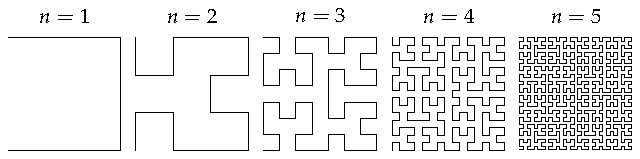
\includegraphics{figures/hilbertcurves.pdf}
    \caption{The first 5 spacefilling Hilbert curves for your enjoyment.}
    \label{fig:hilbert curves}
\end{figure}

\subsection{Tables}
You may know that I like my tables. Use them as floats using the \verb|table| environment. Do not force placement. Always include a caption \emph{above} the table. Don' forget the label using \verb|tab:|. Avoid vertical lines. Minimize horizontal lines (\verb|\toprule|, \verb|\midrule|, \verb|\bottomrule|, essentially). Content alignment: numbers are right aligned (plus decimal aligned, use the siunitx powers for that), text is left aligned. Table headers are aligned like their content. Always refer to tables from the main text, using \verb|\tabref| like the example in \tabref{tab:table with horizontal lines and siunitx for numbers}.

\begin{table}
\caption{This is a neat table: setting up a 6 column table, the first is just left-aligned text, the other 5 columns are decimal-aligned/right, and AUTOMATICALLY ROUNDED to 3 digits after the decimal...}
\label{tab:table with horizontal lines and siunitx for numbers}
\centering
\begin{tabular}{l*{5}{S[table-auto-round=true,table-format=1.3,table-number-alignment=right]}}
    \toprule
    \textbf{Model} & \multicolumn{1}{r}{$f = 10$} & \multicolumn{1}{r}{$20$} & \multicolumn{1}{r}{$50$} & \multicolumn{1}{r}{$100$} & \multicolumn{1}{r}{$200$} \\ \midrule
    \textbf{SVD} & 0.9140 & 0.9074 & 0.9046 & 0.9025 & 0.9009 \\ 
    \textbf{SVD++} & 0.9131 & 0.9032 & 0.8952 & 0.8924 & 0.8911 \\
    \textbf{timeSVD++} & 0.8971 & 0.8891 & 0.8824 & 0.8805 & 0.8799 \\
    \bottomrule
    \end{tabular}
\end{table}


\subsection{Math}
When typesetting math, use inline $f(x)=\sin(x)$, or displayed equations using \verb|\begin{equation}| and \verb|\end{equation}|; this will number the equation even if we don't refer to it later. Avoid empty lines before/after an equation unless you actually desire a new paragraph. Give meaningful labels (\verb|eq:...|) and refer to equations using \verb|\eqref|. For example, we have 
\begin{equation}\label{eq:Eulers law}
  e^{i\pi}+1=0
\end{equation}
and can then refer to it as \eqref{eq:Eulers law}.
A few rules: scalars are just lower case letters (typically latin, except for parameters and angles, where we use greek letters). Matrices are uppercase latin or greek, for vectors use \verb|\vec| (which currently defaults to bold) and lower-case latin letters. Use \verb|\left\langle| and \verb|\right\rangle| for inner products, or \verb|^\top| for the transpose notation:
\begin{equation}
    a = \left\langle \vec{x}, A\vec{x}\right \rangle = \vec{x}^\top A\vec{x}.
\end{equation}


\subsection{Numbers and units}
We will use the power of siunitx for everything numbers and units. For example compare $100,000$ against \num{100000} and tell me which one looks better... or in math mode: $N = \num{100000}$. You can specify ranges all day long, especially \numrange{9}{5}. And units can be typeset at the speed of light \qty{3e5}{\meter\per\second}.

\subsection{Plots}
Exporting plots using \verb|matlab2tikz| or the equivalent for R just looks so much nicer (ey, Jacob Munson?). Keep charts ``empty''. See an example in \figref{fig:png chart not so nice} and compare against the tidy version in \figref{fig:tikz chart very nice}.

\begin{figure}
    \begin{minipage}[t]{.49\textwidth}    
    \centering
    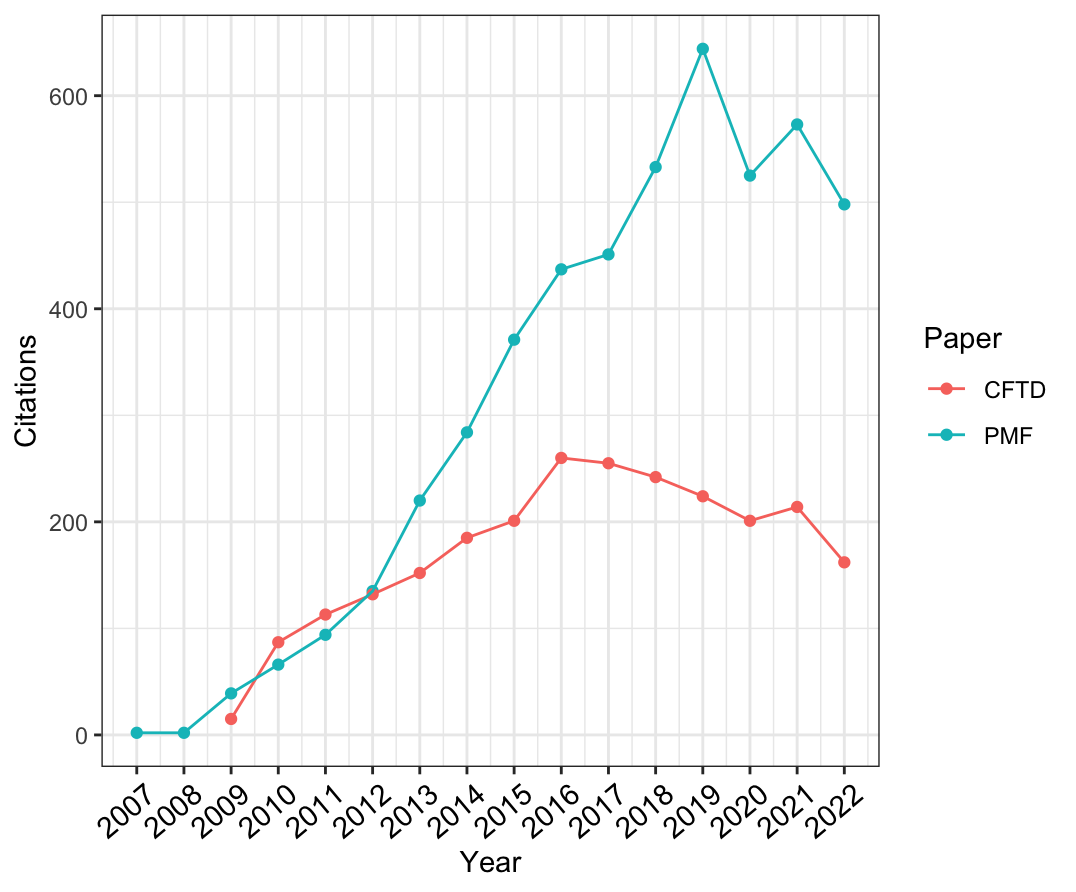
\includegraphics[width=\textwidth]{figures/image.png}
        \caption{Example of a chart exported as a .png file. Notice how the fonts etc. do not correspond to the rest of the document, and the resolution might be bad.}
    \label{fig:png chart not so nice}
    \end{minipage}\hfill
    \begin{minipage}[t]{.49\textwidth}    
    \centering
    % Created by tikzDevice version 0.12.3.1 on 2023-01-22 16:55:02
% !TEX encoding = UTF-8 Unicode
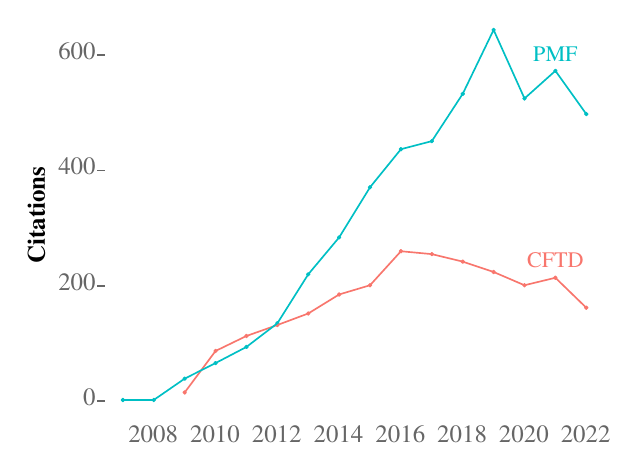
\begin{tikzpicture}[x=0.3pt,y=0.5pt]
%\path[draw,use as bounding box] (-50,0) rectangle (647,361.35);
\begin{scope}

\definecolor{drawColor}{RGB}{0,191,196}
\definecolor{fillColor}{RGB}{0,191,196}

\path[draw=drawColor,line width= 0.4pt,line join=round,line cap=round,fill=fillColor] ( 64.02, 57.87) ellipse [x radius=2,y radius=1.2];

\path[draw=drawColor,line width= 0.4pt,line join=round,line cap=round,fill=fillColor] (101.23, 57.87) ellipse [x radius=2,y radius=1.2];

\path[draw=drawColor,line width= 0.4pt,line join=round,line cap=round,fill=fillColor] (138.44, 73.28) ellipse [x radius=2,y radius=1.2];

\path[draw=drawColor,line width= 0.4pt,line join=round,line cap=round,fill=fillColor] (175.65, 84.53) ellipse [x radius=2,y radius=1.2];

\path[draw=drawColor,line width= 0.4pt,line join=round,line cap=round,fill=fillColor] (212.86, 96.19) ellipse [x radius=2,y radius=1.2];

\path[draw=drawColor,line width= 0.4pt,line join=round,line cap=round,fill=fillColor] (250.07,113.27) ellipse [x radius=2,y radius=1.2];

\path[draw=drawColor,line width= 0.4pt,line join=round,line cap=round,fill=fillColor] (287.28,148.68) ellipse [x radius=2,y radius=1.2];

\path[draw=drawColor,line width= 0.4pt,line join=round,line cap=round,fill=fillColor] (324.49,175.35) ellipse [x radius=2,y radius=1.2];

\path[draw=drawColor,line width= 0.4pt,line join=round,line cap=round,fill=fillColor] (361.70,211.59) ellipse [x radius=2,y radius=1.2];

\path[draw=drawColor,line width= 0.4pt,line join=round,line cap=round,fill=fillColor] (398.91,239.09) ellipse [x radius=2,y radius=1.2];

\path[draw=drawColor,line width= 0.4pt,line join=round,line cap=round,fill=fillColor] (436.12,244.92) ellipse [x radius=2,y radius=1.2];

\path[draw=drawColor,line width= 0.4pt,line join=round,line cap=round,fill=fillColor] (473.33,279.08) ellipse [x radius=2,y radius=1.2];

\path[draw=drawColor,line width= 0.4pt,line join=round,line cap=round,fill=fillColor] (510.54,325.32) ellipse [x radius=2,y radius=1.2];

\path[draw=drawColor,line width= 0.4pt,line join=round,line cap=round,fill=fillColor] (547.75,275.75) ellipse [x radius=2,y radius=1.2];

\path[draw=drawColor,line width= 0.4pt,line join=round,line cap=round,fill=fillColor] (584.96,295.74) ellipse [x radius=2,y radius=1.2] node[above,color=drawColor] {\footnotesize PMF};

\path[draw=drawColor,line width= 0.4pt,line join=round,line cap=round,fill=fillColor] (622.17,264.50) ellipse [x radius=2,y radius=1.2];
\definecolor{drawColor}{RGB}{248,118,109}
\definecolor{fillColor}{RGB}{248,118,109}

\path[draw=drawColor,line width= 0.4pt,line join=round,line cap=round,fill=fillColor] (138.44, 63.28) ellipse [x radius=2,y radius=1.2];

\path[draw=drawColor,line width= 0.4pt,line join=round,line cap=round,fill=fillColor] (175.65, 93.28) ellipse [x radius=2,y radius=1.2];

\path[draw=drawColor,line width= 0.4pt,line join=round,line cap=round,fill=fillColor] (212.86,104.11) ellipse [x radius=2,y radius=1.2];

\path[draw=drawColor,line width= 0.4pt,line join=round,line cap=round,fill=fillColor] (250.07,112.02) ellipse [x radius=2,y radius=1.2];

\path[draw=drawColor,line width= 0.4pt,line join=round,line cap=round,fill=fillColor] (287.28,120.36) ellipse [x radius=2,y radius=1.2];

\path[draw=drawColor,line width= 0.4pt,line join=round,line cap=round,fill=fillColor] (324.49,134.10) ellipse [x radius=2,y radius=1.2];

\path[draw=drawColor,line width= 0.4pt,line join=round,line cap=round,fill=fillColor] (361.70,140.77) ellipse [x radius=2,y radius=1.2];

\path[draw=drawColor,line width= 0.4pt,line join=round,line cap=round,fill=fillColor] (398.91,165.35) ellipse [x radius=2,y radius=1.2];

\path[draw=drawColor,line width= 0.4pt,line join=round,line cap=round,fill=fillColor] (436.12,163.26) ellipse [x radius=2,y radius=1.2];

\path[draw=drawColor,line width= 0.4pt,line join=round,line cap=round,fill=fillColor] (473.33,157.85) ellipse [x radius=2,y radius=1.2];

\path[draw=drawColor,line width= 0.4pt,line join=round,line cap=round,fill=fillColor] (510.54,150.35) ellipse [x radius=2,y radius=1.2];

\path[draw=drawColor,line width= 0.4pt,line join=round,line cap=round,fill=fillColor] (547.75,140.77) ellipse [x radius=2,y radius=1.2];

\path[draw=drawColor,line width= 0.4pt,line join=round,line cap=round,fill=fillColor] (584.96,146.18) ellipse [x radius=2,y radius=1.2] node[above,color=drawColor] {\footnotesize CFTD};

\path[draw=drawColor,line width= 0.4pt,line join=round,line cap=round,fill=fillColor] (622.17,124.52) ellipse [x radius=2,y radius=1.2];

\path[draw=drawColor,line width= 0.6pt,line join=round] (138.44, 63.28) --
	(175.65, 93.28) --
	(212.86,104.11) --
	(250.07,112.02) --
	(287.28,120.36) --
	(324.49,134.10) --
	(361.70,140.77) --
	(398.91,165.35) --
	(436.12,163.26) --
	(473.33,157.85) --
	(510.54,150.35) --
	(547.75,140.77) --
	(584.96,146.18) --
	(622.17,124.52);
\definecolor{drawColor}{RGB}{0,191,196}

\path[draw=drawColor,line width= 0.6pt,line join=round] ( 64.02, 57.87) --
	(101.23, 57.87) --
	(138.44, 73.28) --
	(175.65, 84.53) --
	(212.86, 96.19) --
	(250.07,113.27) --
	(287.28,148.68) --
	(324.49,175.35) --
	(361.70,211.59) --
	(398.91,239.09) --
	(436.12,244.92) --
	(473.33,279.08) --
	(510.54,325.32) --
	(547.75,275.75) --
	(584.96,295.74) --
	(622.17,264.50);
\end{scope}
\begin{scope}
\definecolor{drawColor}{gray}{0.4}

\node[text=drawColor,anchor=base east,inner sep=0pt, outer sep=0pt] at ( 31.16, 54.00) {\small 0};

\node[text=drawColor,anchor=base east,inner sep=0pt, outer sep=0pt] at ( 31.16,137.32) {\small 200};

\node[text=drawColor,anchor=base east,inner sep=0pt, outer sep=0pt] at ( 31.16,220.64) {\small 400};

\node[text=drawColor,anchor=base east,inner sep=0pt, outer sep=0pt] at ( 31.16,303.96) {\small 600};
\end{scope}
\begin{scope}
\definecolor{drawColor}{gray}{0.4}

\path[draw=drawColor,line width= 0.6pt,line join=round] ( 33.36, 57.03) --
	( 42.11, 57.03);

\path[draw=drawColor,line width= 0.6pt,line join=round] ( 33.36,140.35) --
	( 42.11,140.35);

\path[draw=drawColor,line width= 0.6pt,line join=round] ( 33.36,223.67) --
	( 42.11,223.67);

\path[draw=drawColor,line width= 0.6pt,line join=round] ( 33.36,306.99) --
	( 42.11,306.99);
\end{scope}

\begin{scope}
\definecolor{drawColor}{gray}{0.4}

%\node[text=drawColor,inner sep=0pt, outer sep=0pt] at ( 71.28, 33.41) {\small 2007}; rotate= 40.00,anchor=base east,

\node[text=drawColor,inner sep=0pt, outer sep=0pt] at (100.49, 33.41) {\small 2008};

%\node[text=drawColor,inner sep=0pt, outer sep=0pt] at (145.70, 33.41) {\small 2009};

\node[text=drawColor,inner sep=0pt, outer sep=0pt] at (174.91, 33.41) {\small 2010};

%\node[text=drawColor,inner sep=0pt, outer sep=0pt] at (220.12, 33.41) {\small 2011};

\node[text=drawColor,inner sep=0pt, outer sep=0pt] at (249.33, 33.41) {\small 2012};

%\node[text=drawColor,inner sep=0pt, outer sep=0pt] at (294.54, 33.41) {\small 2013};

\node[text=drawColor,inner sep=0pt, outer sep=0pt] at (323.75, 33.41) {\small 2014};

%\node[text=drawColor,inner sep=0pt, outer sep=0pt] at (368.96, 33.41) {\small 2015};

\node[text=drawColor,inner sep=0pt, outer sep=0pt] at (398.17, 33.41) {\small 2016};

%\node[text=drawColor,inner sep=0pt, outer sep=0pt] at (443.38, 33.41) {\small 2017};

\node[text=drawColor,inner sep=0pt, outer sep=0pt] at (472.59, 33.41) {\small 2018};

%\node[text=drawColor,inner sep=0pt, outer sep=0pt] at (517.80, 33.41) {\small 2019};

\node[text=drawColor,inner sep=0pt, outer sep=0pt] at (547.01, 33.41) {\small 2020};

%\node[text=drawColor,inner sep=0pt, outer sep=0pt] at (592.22, 33.41) {\small 2021};

\node[text=drawColor,inner sep=0pt, outer sep=0pt] at (621.43, 33.41) {\small 2022};
\end{scope}

\begin{scope}
\definecolor{drawColor}{RGB}{0,0,0}

\node[text=drawColor,rotate= 90.00,anchor=base,inner sep=0pt, outer sep=0pt] at ( -30,191.59) {\small \textbf{Citations}};
\end{scope}
\end{tikzpicture}
    \caption{Compare the .png against this version that was both tidied up and exported using tikz. The huge advantage of tikz is that we can edit figures while writing the paper, and don't necessarily have to go back to MATLAB/R.}
    \label{fig:tikz chart very nice}
    \end{minipage}
\end{figure}

\section{Code and experiments}
TBD.

\section{Data}
TBD.

\section{Outlook}
We'll probably have to add to these rules as more ``problems'' come up.

%%%%%%%%%%%%%%%%%%%%%%%%%%%%%%%%%%%%%%%%%%%%%%%%%%%%%%%%%%%%%%%%%%%%%%%%%%%%%%%%%%%%%%%%%%%%%%%%%%%%%%%%%%%%%%%%%%%%%%%%%%%%%%%%%%%%
\bibliographystyle{ieeetr}
\bibliography{references}

\end{document}